\section{Transport Protocols and Mobility Choices for ABR Streaming: Performance vs Energy Efficiency}
Any ABR takes the decision based on the directly or indirectly observed network throughput. However, this throughput highly depends on the underlying transport protocol QUIC or TCP. As all the ABR algorithms are primarily designed keeping TCP as the transport protocol in mind, we want to know if those existing ABR algorithm can work fine with the QUIC or other set of algorithms are required. On the other hand, an ABR algorithm's performance can indirectly impact smartphones' power consumption due to the nature of the radio resource controller (RRC). So we also want to profile energy consumption during video streaming.

\subsection{TCP vs QUIC: YouTube}
YouTube started using QUIC as an alternative to TCP via Google chrome and chromium browsers. Both of these browsers support a command-line flag to enable or disable QUIC during execution. So we play ~175 YouTube videos by enabling and disabling the QUIC and record the HAR and {\tt tcpdump} trace to analyze the performance of TCP and QUIC. 
\subsubsection{Observation}
We want to know if QUIC provides better QoE than TCP or not. So, we look for the three parameters, rebuffering, average quality, and quality switches in our collected traces. Our analysis revealed that the QUIC incurs fewer quality switches than TCP, and the overall quality is better with QUIC than with the TCP. In terms of rebuffering, we observed that QUIC suffers more than TCP with the poor network quality. However, TCP suffers more when network quality is better.

\subsection{TCP vs QUIC: DASH}
In the last subsection, we compared the performances of QUIC and TCP for YouTube videos. However, YouTube does not allow us to change or choose the ABR algorithm. This subsection compares these protocols' performance for modern ABRs like BOLA, MPC, and Pensiev with the open-source DASH-IF player and publicly available network traces to throttle the connection with the help of {\tt mahimahi} tool. In our experiment, we keep the server and the player in the same network and throttle the connection using {\tt mahimahi}. We played ~50 videos of a total of 45 hours of playback time using various ABR algorithm.

\subsubsection{Observation}
Our initial observations showed that the QUIC performs poorly for most scenarios in terms of all the QoE components and the overall QoEs. Fig.~\ref{fig:chap03s2:RebufferTime_n} and Fig.~\ref{fig:chap03s2:QOE_n} depict the observations on rebuffering and QoE.

\begin{figure*}[!h]
%	\begin{minipage}[t]{0.48\linewidth}
%		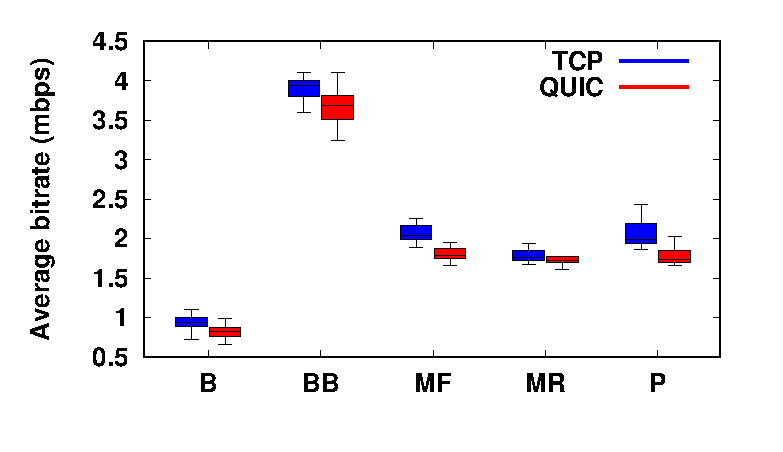
\includegraphics[width=\linewidth]{img/QUIC/bitrate_box}
%		\caption{\label{fig:chap03s2:averageQuality_n}Average Playback Video Quality for Different ABR Techniques ($p<0.05$ for all the metrics)}
%	\end{minipage}\hfill
%	\begin{minipage}[t]{0.48\linewidth}
%		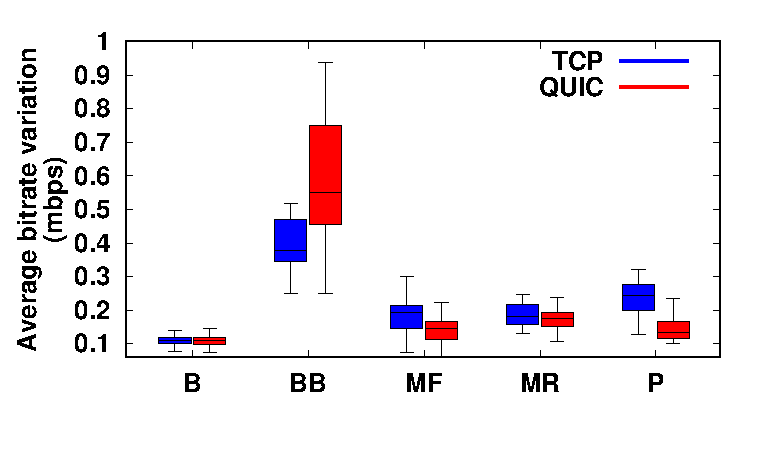
\includegraphics[width=\linewidth]{img/QUIC/smooth_box}
%		\caption{\label{fig:chap03s2:averageQualityVariation_n}Average Playback Quality Variation for Different ABR Techniques ($p<0.05$ for all the metrics except BOLA and MPC-Robust)}
%	\end{minipage}
%	
	\begin{minipage}[t]{0.48\linewidth}
		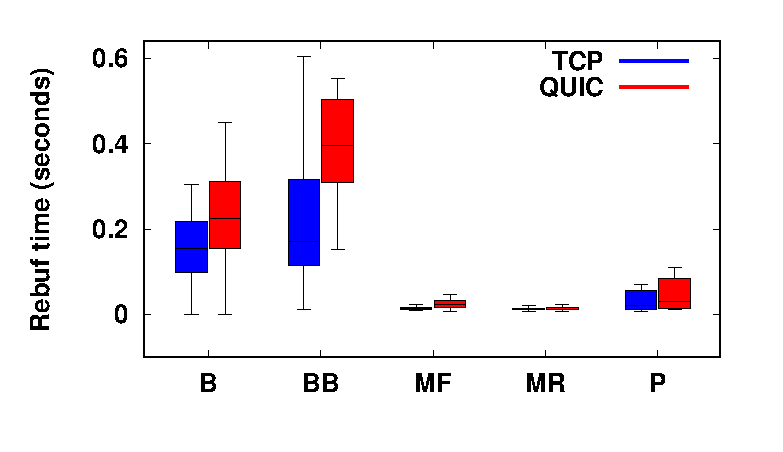
\includegraphics[width=\linewidth]{img/QUIC/rebuf_box}
		\caption{\label{fig:chap03s2:RebufferTime_n}Rebuffering Time for Different ABR Techniques ($p<0.05$ for all the metrics except Pensieve and MPC-Robust)}
	\end{minipage}\hfill
	\begin{minipage}[t]{0.48\linewidth}
		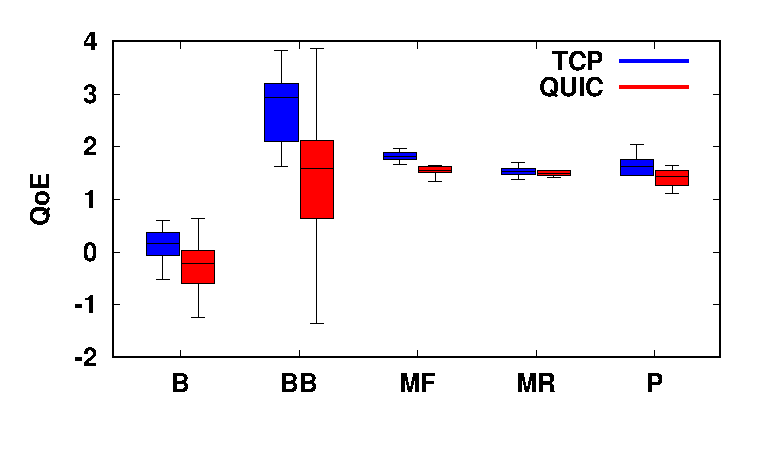
\includegraphics[width=\linewidth]{img/QUIC/qoe_box}
		\caption{\label{fig:chap03s2:QOE_n}Overall QoE for Different ABR Techniques ($p<0.05$ for all the metrics except MPC-Robust)}
	\end{minipage}
\end{figure*}

\subsection{Energy Consumption due to ABR Streaming: An Experimental Analysis}
We wanted to profile the energy consumption by ABR streaming. So, we experiment with commodity smartphones on our campus. We move around our campus with a slow-moving vehicle and collect GPS, radio parameters from the smartphone. We also collect energy consumption traces using the monsoon power monitor tool to perform the experiments. In this setup, two mainly performed two experiments, a) downloaded files from a server and b) played YouTube videos.
\subsubsection{Observations}
From these experiment we find two takeaways: a) the wireless network condition is best quantified by throughput which depends significantly on phenomena such as handovers and not on received signal quality alone, and b) the current protocol of video download attributes a higher weightage to the playback-buffer length than the user’s instantaneous received signal strength or throughput, ensuing a significantly high energy consumption.